\documentclass[runningheads]{llncs}
\usepackage[T1]{fontenc}

\usepackage{graphicx}

\usepackage{color}
\usepackage{xcolor}
\definecolor{red}{cmyk}{0,1,0.9,0.3}
\definecolor{green}{cmyk}{0.9,0,0.7,0.5}

\usepackage{url}
\usepackage{hyperref}
\renewcommand\UrlFont{\color{blue}\rmfamily}
\urlstyle{rm}

\usepackage{tikz}
\usepackage{pgfplots}
\usepackage{pgfplotstable}
\pgfplotsset{compat=1.18}
\pgfkeys{/pgf/number format/.cd,fixed,precision=0}
\pgfplotstableset{col sep=comma}

\usepackage{listings}
\lstdefinelanguage{red}[]{}{%
    keywords={},
    otherkeywords={},
    basicstyle=\color{red}\fontsize{8}{8}\selectfont\ttfamily
}
\lstdefinelanguage{SaC}[]{}{%
    keywords={typedef,char,byte,int,float,double,bool,inline,return,dim,shape,take,drop,floor,sqrt,pow3,rsum,struct,class,temperature,Vector3,Body,reverse,reshape,dummy},
    otherkeywords={?,:},%->,<,<=,>,>=,+,-,*,/,^,+=,-=,*=,/=,==},
    moredelim=[s][\color{green}]{/*}{*/},
    morecomment=[s]{Body[}{]},
    morecomment=[s]{double[}{]},
    morecomment=[s]{[:}{]},
    morecomment=[s]{type}{]}
}
\lstset{%
    language=SaC,
    basicstyle=\fontsize{8}{8}\selectfont\ttfamily,
    keywordstyle=\color{blue},
    commentstyle=\color{blue},
    showstringspaces=false,
}
\newcommand{\sub}[1]{\textsubscript{#1}}
\newcommand{\subb}[1]{{\color{blue}\sub{#1}}}

% ----------------------------------------------------------------------

\newcommand{\sac}{SaC}

% Highlight a piece of text into a gray block
\definecolor{highlight}{cmyk}{0,0,0,0.12}
\newcommand{\highlight}[1]{\colorbox{highlight}{$\displaystyle #1$}}

%
% A bunch of commands to make the translation formulas consistent and easier to change
%

\newcommand{\recordtype}[1]{\text{struct #1}}
\newcommand{\recorddecl}[2]{\recordtype{#1}\ \{\,#2\,\};}
\newcommand{\recordvar}[2]{\recordtype{#1}\ #2}

\newcommand{\idN}[2][field]{\textit{#1}_{#2}}
\newcommand{\typeN}[1]{\textit{type}_{#1}[\textit{shp}_{#1}]}
\newcommand{\fieldN}[2][field]{\typeN{#2}\ \idN[#1]{#2}}

\newcommand{\us}{\ensuremath{\mathunderscore{}}}
\newcommand{\rtCon}{\text{\us{}rt\us{}constr\us{}}}
\newcommand{\rtGet}[2][]{\text{\us{}rt\us{}get\us{}#2\textsubscript{#1}\us{}}}
\newcommand{\rtSet}[2][]{\text{\us{}rt\us{}set\us{}#2\textsubscript{#1}\us{}}}

\newcommand{\denest}[2][\sigma]{\texttt{Denest}(#2,\ #1)}
\newcommand{\denestRT}[2][\sigma]{\texttt{Denest\textsubscript{rt}}(#2,\ #1)}
\newcommand{\expand}[2]{\texttt{expand}(#1,\ #2)}
\newcommand{\envsub}[1]{\ensuremath{\sigma_{\text{#1}}}}
\newcommand{\envid}[2][]{\text{#2\textsubscript{#1}:}\;}
\newcommand{\makeenv}[1]{\{\,#1\,\}}

% ----------------------------------------------------------------------

\title{Flattening Combinations of Arrays and Records}

\author{Reg Huijben
   \and Jordy Aaldering\orcidID{0009-0001-3018-5152}
   \and Peter Achten\orcidID{0000-0002-3585-7165}
   \and Sven-Bodo Scholz\orcidID{0000-0002-8663-1043}}

\institute{Radboud University, Nijmegen, Netherlands \\
\email{\{Reg.Huijben,Jordy.Aaldering,Peter.Achten,SvenBodo.Scholz\}@ru.nl}}

\begin{document}
\maketitle


\begin{abstract}
In this paper we present type patterns: a notation for shape-carrying array types that enables the specification of dependent type signatures while maintaining flexibility and a high level of code readability.
Similar notations pre-exist, but we extend them to support rank-polymorphism and specifications of arbitrarily complex constraints between values and types.
Furthermore, we enable type patterns to double as a pattern matching mechanism against shapes and shape-components of array arguments, making those values directly available in the corresponding function bodies.

While this notation could be used as a basis for a dependently typed language, in our prototypical implementation in the context of SaC we do not require all dependencies to be resolved statically.
Instead, we follow a hybrid approach:
we map the proposed type patterns into the pre-existing type system of SaC, and we generate additional constraints which we try to statically resolve as far as possible by means of partial evaluation.
Any remaining constraints are checked at run-time.
We outline our implementation in the context of the SaC ecosystem, and present several examples demonstrating the effectiveness of this hybrid approach based on partial evaluation.
\end{abstract}


\section{Introduction}

The importance of software sustainability has grown rapidly in recent years, alongside an increasing
awareness of environmental concerns. From mobile applications to data centres, minimizing the energy
consumption of software has become essential for mitigating environmental impact, increasing battery
life, and reducing operational costs. Traditional software systems often focus on maximizing runtime
performance without adequately considering energy consumption. However, as sustainability becomes a
priority, there is a growing need for approaches that balance runtime performance and
energy-efficiency.

The current landscape of computing hardware is characterized by its heterogeneity, with a shift
towards multicore and many-core systems. High-perfor\-mance computing applications typically aim to
fully utilize all available resources on these systems, with the goal of maximizing runtime
performance. Determining efficient resource allocation for optimizing performance -- be it runtime
or energy-efficiency -- depends not only on an algorithm's implementation, but also on input data
size, hardware characteristics, cache utilization, and system-specific configurations such as thread
pinning. This makes static approaches for determining resource allocation increasingly difficult, as
they fail to account for variations in hardware capabilities~\cite{heterogeneous-systems}.
Furthermore, it has been shown that optimizing for runtime is not always equivalent to optimizing
for energy-efficiency, and that optimizing runtime can have a negative effect on energy
consumption~\cite{compiler-energy-android,compiler-energy-differences}.

A key candidate for improving the energy-efficiency through more efficient resource allocation is
the thread management of an application. Traditionally, thread management in software systems has
focused primarily on performance metrics such as execution time and operations per second. A notable
approach in the context of the Single assignment C (\sac{}) language uses a dynamic adaptation
algorithm that adjusts the thread-count of a program by observing changes in runtime
metrics~\cite{sac-mtdynamic}. This technique enables \sac{} applications to adapt to varying
workloads and resource availability, improving runtime performance by efficiently utilizing
computational resources. This method optimizes for runtime performance, but does not directly
address energy consumption.

We present a method that extends existing runtime adaptation techniques by incorporating energy
consumption as the primary factor in decision-making. By dynamically adjusting the number of threads
based on real-time energy consumption metrics, we show that it is possible to achieve a more
sustainable balance between runtime performance and energy-efficiency. Functional languages are an
especially suitable target for this dynamic adaptation algorithm, as their side-effect-free nature
and strong semantic guarantees allow for easier code generation and straightforward scalability of
the parallelism of programs.

Our contributions are:
\begin{itemize}
    \item A static analysis of data-parallel programs that investigates the relation between the
    level of parallelism and overall energy consumption. (Section~\ref{sec:observations})
    \item A dynamic adaptation algorithm that aims to minimize energy consumption of data-parallel
    programs at runtime through external control. (Section~\ref{sec:implementation})
    \item An implementation of a thread-steering mechanism in the data-parallel functional language
    \sac{}, based on this adaptation algorithm. (Section~\ref{sec:implementation-sac})
    \item An evaluation of how close the adaptation algorithm comes to the energy-efficiency of a
    theoretical optimum. (Section~\ref{sec:evalation-adaptation} and \ref{sec:evalation-oracle})
    \item An evaluation of the energy-efficiency of the adaptation algorithm compared a
    runtime-based approach and static approaches. (Section~\ref{sec:evalation-runtime} and
    \ref{sec:evalation-static})
\end{itemize}


\section{Single assignment C}\label{sec:sac}

Since we use the functional array language Single~assignment~C (\sac{})~\cite{sac,sac2} as implementation vehicle for our proposed flattening,
we provide a quick overview of the key features that we use throughout the paper.
For a more in-depth introduction we refer the reader to papers such as~\cite{sac,sac2} or the online material available on \url{https://sac-home.org/docs:main}.

\sac{} combines a syntax very close to the imperative language C with a purely
side-effect-free semantics. This is achieved by the addition of multi-dimensional, immutable arrays to the language core, paired with an exclusion of pointers.

\subsection{Arrays in \sac{}}

Arrays in \sac{} are multi-dimensional; each array has a dimensionality (also referred to as \textit{rank}) and a \textit{shape} which describes the legal index-space of the array.
This enables computations on multi-dimensional arrays to inspect and 
manipulate not only the data of an array but also its rank and shape.
Table~\ref{tab:array} shows a few examples for arrays in \sac{}. The left-most column provides
an abstract / mathematical representation, the middle column contains a corresponding definition in \sac{} and in the right column we see the three conceptual components of these arrays: their rank (an integer value), their shape (a vector of natural numbers), and their data (a vector of the values of the array). 

\begin{table}[ht!]
    \newcommand{\repr}[3]{%
        \begin{tabular}{ll}
            rank:  & #1   \\
            shape: & [#2] \\
            data:  & [#3]
        \end{tabular}\vspace{2pt}\\\hline\noalign{\vskip 2pt}}
    \centering
    \begin{tabular}{c@{\hskip 1em}c@{\hskip 1em}l}\hline\noalign{\vskip 2pt}
        $\begin{pmatrix}
            1 & 2 & 3 \\
            4 & 5 & 6 \\
            7 & 8 & 9
        \end{pmatrix}$
            & \texttt{[[1,2,3], [4,5,6], [7,8,9]]}
            & \repr{2}{3,3}{1,2,3,4,5,6,7,8,9}
        $\begin{pmatrix}
            1, & 2, & 3, & -4, & -5
        \end{pmatrix}$
            & \texttt{[1,2,3,-4,-5]}
            & \repr{1}{5}{1,2,3,-4,-5}
        $\begin{pmatrix}\begin{pmatrix}
            true, & false, & true
        \end{pmatrix}\end{pmatrix}$
            & \texttt{[[true, false, true]]}
            & \repr{2}{1,3}{true,false,true}
        0.5 
            & \texttt{0.5}
            & \repr{0}{\,}{0.5}
    \end{tabular}
    \caption{Array representation in \sac{}}
    \label{tab:array}
\end{table}

\noindent
From this table, we can observe that all elements of any given array ultimately can be represented as a \textit{flat} data vector in memory.
While the \sac{} syntax in the middle column may suggest to the programmer that some arrays indeed are nested, in fact, they are not; in \sac{}, nesting inherently is indistinguishable from higher-dimensional arrays.
This contrasts starkly with the idea of arrays prevalent in most non-array languages, where arrays are considered inherently one dimensional and where higher dimensional arrays are mimicked through nesting.
As a consequence of \sac{}'s choice to support higher-dimensional arrays in combination with a vector for representing the shape, nested notations in \sac{} are restricted to the homogeneous case, i.e. all inner expressions must have the same shape.
An expression of the form \texttt{[[1],\,[2,3]]} is not admissible in \sac{}.

\subsection{Tensor Comprehensions}

The key language construct of \sac{} for defining arrays from other arrays is the \textit{Tensor Comprehension}~\cite{sac-tensor,sac-scan}.
A tensor comprehension is essentially a mapping of index vectors to values.
For example, the tensor comprehension
%
\begin{lstlisting}
{ iv -> arr[iv] * 2  |  iv < shape(arr) }
\end{lstlisting}
%
defines an array of the same shape as array \texttt{arr}, whose value in each index position \texttt{iv} equates to twice the value of \texttt{arr} at the given position.
Note here that the index variable \texttt{iv} denotes an index vector with as many elements as the array \texttt{arr} has dimensions.
The ability to express such operations that operate on arrays of arbitrary rank is referred to as \textit{rank polymorphism}.
If a fixed rank is expected, an explicit vector of indices can be used instead.
For example,
%
\begin{lstlisting}
{ [i,j] -> mat[j,i]  |  [i,j] < reverse(shape(mat)) }
\end{lstlisting}
%
transposes the two dimensional array \texttt{mat}.
Despite having a fixed-rank index space, this tensor comprehension can be turned into a rank polymorphic operation by a small change into
%
\begin{lstlisting}
{ [i,j] -> mat[j,i]  |  [i,j] < reverse(take([2], shape(mat))) }
\end{lstlisting}
%
The rank polymorphism of this expression is achieved through two measures.
Firstly, selections in \sac{} select entire subarrays if there are fewer indices than the rank of the array to be selected from.
Secondly, the specification of the upper bound through \texttt{reverse(take([2], shape(mat)))} ensures a two element vector as upper bound, even if the rank of the array \texttt{mat} is higher than 2.

\subsection{Function Definitions, Types, and Type Patterns}

Function definition in \sac{} look like their C counterparts.
The main difference is the types that are supported in \sac{}.
All types in \sac{} consist of an element type followed by a shape specification.
If the shape specification is omitted, scalar arrays are expected.
For example, the simple transpose can be defined as:
%
\begin{lstlisting}
double[n,m] transpose(double[m,n] mat)
{
    return { [i,j] -> mat[j,i]  |  [i,j] < reverse(shape(mat)) };
}
\end{lstlisting}
%
Note here that the shape variables \texttt{m} and \texttt{n} define scalar integer values that can be referred to in the function body.
This allows for a specification of the upper bound as \texttt{[n,m]} instead of \texttt{reverse(shape(mat))}.
%
\begin{lstlisting}
double[n,m] transpose(double[m,n] mat)
{
    return { [i,j] -> mat[j,i]  |  [i,j] < [n,m] };
}
\end{lstlisting}
%
The dual use of shape variables for describing domain constraints as well as for capturing these values are referred to as \textit{type patterns}~\cite{sac-typepattern}.


\section{Introducing type patterns}

We introduce type patterns from the perspective of introducing a pattern matching mechanism, as this matches more directly with the way we map them into the pre-existing hybrid type system of SaC.
An alternative way to think about type patterns is to see them as ways to introduce types, through the introduction of variables within type signatures of function definitions.

\subsection{Syntax of type patterns}

We start out with the syntax of type patterns, shown in Figure~\ref{fig:syntax}.

\begin{figure}[hbt]
\begin{verbatim}
<pattern>  ::= <type> '[' <feature> (',' <feature>)* ']'

<feature>  ::= <single>
            |  <multiple>

<single>   ::= '.'
            |  <num>
            |  <id>

<multiple> ::= '*'
            |  '+'
            |  <num> ':' <id>
            |  <id> ':' <id>
\end{verbatim}
\caption{EBNF for type patterns}
\label{fig:syntax}
\end{figure}

\noindent
This syntax extends of the notion of array types from SaC, providing more syntactical flexibility and introducing variables within these types.
Similar to the types in SaC, type patterns consist of an element type followed by a shape specification in square brackets.
The shape specification is a pattern, which consists of a list of `features'.
These features either describe a single rank of the argument, or a larger slice (a sub-vector) of its shape vector.

Single dimensions are captured by the \verb|<single>| rule in Figure~\ref{fig:syntax} and can be denoted by the `\tpdot{}' symbol, a constant number, or a variable name. 
A fixed number requires the length of the corresponding rank component to match that very number, whereas the `\texttt{.}' symbol allows for an arbitrary extent.
If instead a variable is being used, the extent found needs to match all other occurrences of that very variable within a given function definition.
For example, consider the type pattern \texttt{int[n,n]}.
It allows for square matrices of arbitrary size $\texttt{n} \times \texttt{n}$ where \texttt{n} is a non-negative integer value.

Rank-polymorphism requires the ability to denote a statically unknown number of ranks.
To cater for this, the proposed type patterns support features that capture slices of a given shape.
These are captured by the \verb|<multiple>| rule in Figure~\ref{fig:syntax}.
We distinguish four cases, depending on the rank of the slice we want to match, and whether we are interested in the slice itself or not.
If we are not interested in the slice itself, we can use one of the symbols `\texttt{+}' and `\texttt{*}'.
They match any slice of at least rank 1 or 0, respectively.

If we are interested in the slice itself, the feature consists of two components separated by a `\texttt{:}' symbol.
The first component relates to the rank of that slice, whereas the second component relates to the slice itself, i.e. the lengths of the corresponding axes.
For the rank component, similar to the single-rank features, we can either use a fixed number or an identifier.
For example, \texttt{int[3:shp]} matches rank 3 arrays only, and matches the entire shape vector against the variable \texttt{shp} that will thus be a three-element vector.
Note here that variables after the `\texttt{:}' symbol, such as \texttt{shp}, denote slices and therefore always represent vectors, even if they match no ranks (empty vector) or individual ranks (singleton vector).
For example, a type pattern \texttt{int[1:n,1:n]}, similar to the \texttt{int[n,n]} example above, matches arbitrary sized square matrices, but \texttt{n} now is a singleton vector rather than a scalar value. 

Finally we have the case where the rank of the slice is also a variable, enabling a match of a variable-rank slice of an array shape.
Here, the first component matches against the rank of the slice, and the second component again matches against the slice itself.
For example, the pattern \texttt{int[d:shp]} matches arrays of arbitrary shape, and binds the variable \texttt{d} to the rank of the array, and the variable \texttt{shp} to the shape of the array.

These features can be combined to create complex type patterns.
Consider for example a type pattern \texttt{int[5,n,d:shp]} \texttt{v}.
It matches any shape of at least rank 2, whose extent in the first axis is exactly five, and whose extent in the second axis is \texttt{n}.
Any potentially remaining axes are bound to the vector \texttt{shp}.
These variables (\texttt{n}, \texttt{d}, and \texttt{shp}) can also be used in the function body.
Following are some examples for arguments \texttt{v} and the resulting values of \texttt{n}, \texttt{d}, and \texttt{shp}.

\begin{table}[ht!]
\ttfamily
\begin{tabular}{lllll}\hline
    shape(v)             & 5 & n & d & shp       \\\hline
    \text{}[5,1]         & 5 & 1 & 0 & []        \\
    \text{}[5,1,7]       & 5 & 1 & 1 & [7]       \\
    \text{}[5,0,1,2]     & 5 & 0 & 2 & [1,2]     \\
    \text{}[5,2,1,2,3,4] & 5 & 2 & 4 & [1,2,3,4] \\\hline
\end{tabular}
\end{table}

\noindent
Variable names may be used more than once.
For example, the variable \texttt{n} can be reused in a variable-rank feature \texttt{[5,n,n:shp]}~\texttt{v}.
This pattern matches arrays of at least rank 2 whose extent in the second axis determines the number of ranks that follow.
Some examples of matching shapes are:

\begin{table}[ht!]
\ttfamily
\begin{tabular}{llll}\hline
    shape(v)             & 5 & n & shp       \\\hline
    \text{}[5,0]         & 5 & 0 & []        \\
    \text{}[5,1,0]       & 5 & 1 & [0]       \\
    \text{}[5,1,42]      & 5 & 1 & [42]      \\
    \text{}[5,4,1,2,3,4] & 5 & 4 & [1,2,3,4] \\\hline
\end{tabular}
\end{table}

\noindent
Note that \texttt{d} in the first example, and \texttt{n} in the second example, are equal to the length of \texttt{shp}, which is always the case for such variable-rank patterns.


\section{Example}\label{sec:example}

As a running real-world example we consider the \textit{naive n-body problem}, which is concerned with predicting the individual motions of a group of celestial bodies.
We define a record \texttt{Body} to keep track of these celestial bodies, as well as a \texttt{Vector3} record for the position of this body.
Using these we define a function that computes the acceleration one body imposes on another, along with a function that computes the acceleration imposed on each body by all other bodies.
%
\begin{lstlisting}
struct Vector3 {
    double x;
    double y;
    double z;
};

struct Body {
    struct Vector3 pos;
    double mass;
};

struct Vector3
acc(struct Body b1, struct Body b2)
{
    dir = b2.pos - b1.pos;
    factor = l2norm(dir) == 0.0
        ? 0.0 : b2.mass / pow3(l2norm(dir));
    return factor * dir;
}

struct Body[n]
acc_v(struct Body[n] bodies)
{
    return { [i] -> rsum(1, { [j] -> acc(bodies[i], bodies[j])
                            | [j] < shape(bodies) })
           | [i] < shape(bodies) };
}
\end{lstlisting}
%
With these acceleration functions we can define a function that computes the updated positions of all bodies after some given delta time \texttt{dt}.
For this each body additionally requires a velocity field, which we can add to the record without requiring modifications to the acceleration function, highlighting one of the benefits of using records.
%
\begin{lstlisting}
struct Body {
    struct Vector3 pos;
    double[3] vel;
    double mass;
};

struct Body[n]
timestep(struct Body[n] bodies, double dt)
{
    acceleration = acc_v(bodies);
    bodies.pos += bodies.vel * dt;
    bodies.vel += acceleration * dt;
    return bodies;
}
\end{lstlisting}


\section{Key Idea}\label{sec:key-idea}

In a typical naively nested memory layout for arrays of records (Fig.~\ref{fig:memory}) each element in the array is a pointer to a single record object, where each of those objects has a single value for each field of that record.
In the case that these fields are arrays or nested records, they are yet again pointers to that array or record object respectively.
Such a naive nesting requires a large amount of memory allocations, and consequently results in a blowup in the amount of reference counting operations that is required.
Furthermore this naive nesting has a negative impact on the memory locality of these objects;
adjacent record fields in an array of records are no longer adjacent in memory.
This limits the applicability of vectorization of operations on arrays of records.

\begin{figure}[ht!]
    \centering
    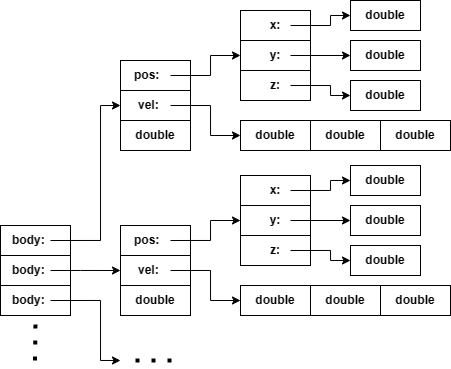
\includegraphics[width=0.7\linewidth]{images/records.png}
    \caption{Naively nested memory layout of the \texttt{Body} record.}
    \label{fig:memory}
\end{figure}

In order to combat these drawbacks we rewrite records into a flattened array representation, where each base-type field is defined by a single array.
Nested records are recursively flattened until only base-types remain.
In the proposed flattened representation, only a single allocation is required for each base-type field of a record.
Consequently this also decreases the amount of reference counting operations that is required, and opens the door to vectorization of operations on these arrays.

This transformation from arrays of records to flattened arrays additionally requires a rewrite of the rest of a program.
Programs need to be rewritten to operate on multiple arrays, instead of on singular arrays of records.
In the case of the n-body example, the record declaration is removed and the acceleration and timestep functions are rewritten to operate on arrays instead.
These functions now require additional arguments and return multiple return values, instead of only a single record.
Unused record fields are removed from these rewritten function definitions. 
Below we show the result of the rewriting process on the acceleration functions from the example.
%
\begin{lstlisting}
double, double, double
acc(double x1, double y1, double z1,
    double x2, double y2, double z2,
    double mass2)
{
    xdir = x2 - x1;
    ydir = y2 - y1;
    zdir = z2 - z1;
    factor = l2norm(xdir, ydir, zdir) == 0.0
        ? 0.0 : m / pow3(l2norm(xdir, ydir, zdir));
    return (xdir * factor, ydir * factor, zdir * factor);
}

double[n], double[n], double[n]
acc_v(double[n] xs, double[n] ys, double[n] zs, double[n] masses)
{
    return { [i] -> rsum(1, { [j] -> acc(xs[i], ys[i], zs[i],
                                         xs[j], ys[j], zs[j],
                                         masses[j])
                            | [j] < [n] })
           | [i] < [n] };
}
\end{lstlisting}
%
The example shows that the transformation is not trivial. 
When arrays and records are combined and nested, the transformation to the required homogeneous arrays by \sac{} can become complex.
To ensure that arrays of records can be transformed into homogeneous arrays we disallow (mutual) recursion and we require that array fields in records are of a statically known and fixed shape.

Additional effort is required for primitive functions, in order for those to be able to operate on record types.
For example, it should be possible to get the dimensionality or shape of an array of records, or to select one of its elements, without the need for a special syntax.
Similarly we need to ensure that tensor comprehensions and other array constructors are able to operate on multiple arguments.
Already in the n-body example we see that often not all fields defined in a record are used by a function, and that not all fields of a record need to be returned.
In order to limit the overhead introduced by an increase in the amount of arguments, and to maximise optimisation potential, two more optimisations are required to remove these unused arguments and return values.



\iffalse
\subsection{Interleaving}

In certain scenarios an interleaved (but flattened) memory layout is actually preferred, as opposed to the suggested flattened notation.
Consider the position field from the body record.

\begin{lstlisting}
struct Body {
    double[3] pos;
    double[3] vel;
    double mass;
}
\end{lstlisting}

Given a vector of these bodies, the positions will become an \texttt{[n,3]} array where the x-y-z coordinates of each position follow each other in memory.
However in the case where we want to apply an operation on only the x-coordinates of a vector of bodies, such a memory layout is not beneficial as the y and z coordinates avoid these operations from being vectorized.
This however can be resolved by expressing the record differently.
Instead of having the position be a three-element vector, it can be represented as a record:

\begin{lstlisting}
struct Pos {
    double x;
    double y;
    double z;
}
\end{lstlisting}

With this notation each coordinate will be expanded into a separate array, now allowing for vectorization of these operations on only the x-coordinates of these bodies.
This example highlights how one can play with the combination of arrays and records in order to obtain the most efficient memory layout.
\fi


\section{Transformation}\label{sec:transform}

Similarly to earlier approaches (Homann et al.~\cite{SoA}, Jubertie et al.~\cite{AoSoA}, Kofler et al.~\cite{AoSoA2}) we aim to improve the runtime performance of programs with records by transforming arrays of records into records of arrays.
However, we go one step further and remove records from programs entirely.
As discussed in Section~\ref{sec:key-idea} this transformation decreases the number of allocations and reference counting operations, as well as improving memory locality.
An additional benefit is that removing records from programs in their entirety decreases the implementation effort of adding records to the language, since no modifications to the type system and other existing compiler phases are necessary.
Especially in a large-scale project such as \sac{}, with many compiler phases that would require modifications to support records, such a transformation is paramount for a feasible implementation effort.

After the record transformation has been applied to a program, that program will no longer contain any record types.
Instead, all record arguments and variable declarations are replaced by distinct arrays.
Record constructors and field accessors and mutators are transformed into functions that operate on arrays instead.
Any user-defined functions and primitive operations on records are similarly transformed into operations on arrays.

In the case of \sac{} this record transformation is actually split up into two separate phases.
During the parsing phase we replace records by a temporary ``external'' type, which is only fully removed after the type checking phase.
This ensures that error messages generated by the type checker still pertain to record types without having to add support for records to the type checker, and that these error messages remain consistent with the pre-existing error messages.
For example we get the following error message if we try to add a body to a string.
%
\begin{lstlisting}[language=red]
No definition found for a function "ArrayArith::+" that accepts
an argument of type "_MAIN::_struct_Body" as parameter no 1.
Full argument types are "( _MAIN::_struct_Body, String::string)".
\end{lstlisting}
%
However had records already been transformed into distinct arrays, the error message would look as follows and the relation between the error and the actual written code would be lost.
%
\begin{lstlisting}[language=red]
No definition found for a function "Array::+" that
expects 4 argument(s) and yields 1 return value(s)
\end{lstlisting}
%
For the sake of brevity however, we omit this additional step in the following transformation rules because it is specific to \sac{} and is not relevant to the actual transformation of records to arrays.

% ----------------------------------------------------------------------


\subsection{Constructors, Accessors, and Mutators}

The first step in transforming programs with records into programs without records is to replace record constructors, accessors, and mutators by generated function definitions.
For each record type in a program we generate a full constructor and a default constructor function, as well as accessor and mutator functions for every field of that record.
Any record constructors, accessors, and mutators in the program are then replaced by applications of the corresponding generated functions.

\subsubsection{Accessors and Mutators}

Normally an infix dot symbol is used to access or mutate the field of a record type, e.g. \texttt{bodies.pos}.
In order to access or mutate a nested field, multiple accessors or mutators may be chained.
However after programs have been transformed there will no longer be any records, and such a selection is no longer applicable.
Instead we generate accessor and mutator functions for every field occurring in a record type.
To access and mutate the position field of the body record, for example, these would be \verb|body_set_pos| and \verb|body_get_pos| respectively.
For a record type with $n$ fields, we generate an accessor and a mutator function for every field $i\in[1,n]$:
%
\begin{lstlisting}[escapechar=$]
type$\subb{1}$[shp$\subb{1}$], ..., type$\subb{n}$[shp$\subb{n}$]
rt_get_id$\sub{i}$(type$\subb{1}$[shp$\subb{1}$] id$\sub{1}$, ..., typen[shp$\subb{n}$] id$\sub{n}$)
{
    return id$\sub{i}$;
}

type$\subb{1}$[shp$\subb{1}$], ..., type$\subb{n}$[shp$\subb{n}$]
rt_set_id$\sub{i}$(type$\subb{i}$[shp$\subb{i}$] value, type$\subb{1}$[shp$\subb{1}$] id$\sub{1}$, ..., type$\subb{n}$[shp$\subb{n}$] id$\sub{n}$)
{
    return (id$\sub{1}$, ..., id$\sub{i-1}$, value, id$\sub{i+1}$, ..., id$\sub{n}$);
}
\end{lstlisting}
%
Note that the argument and return types in these generated functions can still be records at this point.
We expand these records at a later step, along with the expansion of records in user-defined functions.

Accessors and mutators through field selection can now be replaced by applications of these generated functions.
For a field selection \verb|id = x.y| on the right-hand-side of a let-expression we apply the accessor function \verb|id = rt_get_y(x)|, whereas if on the left-hand-side there occurs a field selection \verb|x.y = expr|, the mutator function is applied \verb|rt_set_y(expr, x)|.

\subsubsection{Constructors}

Syntactically there are three kinds of record constructors:
a full constructor that expects a value for each field in order,
a default constructor that takes no arguments and assigns a default (zero) value to each field,
and an explicit constructor with only the values for some fields explicitly defined.
For every record type \texttt{rt} in the program we generate a new function definition for both the full and the default constructor:
%
\begin{lstlisting}[escapechar=$]
type$\subb{1}$[shp$\subb{1}$], ..., type$\subb{n}$[shp$\subb{n}$]
new_rt(type$\subb{1}$[shp$\subb{1}$] id$\sub{1}$, ..., type$\subb{n}$[shp$\subb{n}$] id$\sub{n}$)
{
    return (id$\sub{1}$, ..., id$\sub{n}$);
}

type$\subb{1}$[shp$\subb{1}$], ..., type$\subb{n}$[shp$\subb{n}$]
zero(type$\subb{1}$[*] id$\sub{1}$, ..., type$\subb{n}$[*] id$\sub{n}$)
{
    return new_rt(genarray([shp$\sub{1}$], zero([:type$\subb{1}$])
                  ...
                  genarray([shp$\sub{n}$], zero([:type$\subb{n}$]));
}
\end{lstlisting}
%
Where \texttt{[:type]} is an empty array of the given type.
This ensures that the correct overload of the \texttt{zero} function is applied, returning the default value for that type.

Now whenever we encounter a full constructor of the form \texttt{rt\{expr\sub{1}, ..., expr\sub{n}\}} we replace it by \texttt{new\_rt(expr\sub{1}, ..., expr\sub{n})}, and whenever we encounter a default constructor of the form \texttt{rt\{\}} we replace it by \texttt{zero([:rt])}.
Finally, if we encounter an explicit constructor of the form
%
\begin{lstlisting}[escapechar=$]
rt{.field$\sub{q}$ = value$\sub{q}$, ..., .field$\sub{r}$ = value$\sub{r}$}
\end{lstlisting}
%
we first apply the default constructor, followed by a chain of mutator functions for the explicitly given fields.
%
\begin{lstlisting}[escapechar=$]
rt_set_id$\sub{r}$(value$\sub{r}$,
    ...
        rt_set_id$\sub{q}$(value$\sub{q}$, zero([:rt]));
\end{lstlisting}


\subsection{Expanding Records to Base Types}\label{sec:expand}

After record-specific syntax has been replaced by function applications, we must ensure that those and all other functions no longer contain any record types and record variables.
To achieve this we replace those record types and variables by the fields of those records instead.
We look at the \texttt{l2norm} function as an example:
%
\begin{lstlisting}
double
l2norm(struct Vector3 v)
{
    vx = vector3_get_x(v);
    vy = vector3_get_y(v);
    vz = vector3_get_z(v);
    return sqrt(vx * vx + vy * vy + vz * vz);
}
\end{lstlisting}
%
We aim to transform this function into one without any record types.
%
\begin{lstlisting}
double
l2norm(double x, double y, double z)
{
    vx = vector3_get_x(x, y, z);
    vy = vector3_get_y(x, y, z);
    vz = vector3_get_z(x, y, z);
    return sqrt(vx * vx + vy * vy + vz * vz);
}
\end{lstlisting}
%
In this example we see how the record argument \texttt{struct Vector3 v} is separated into three distinct arguments x, y, and z; corresponding to the three fields of the \texttt{Vector3} record.
Furthermore, all occurrences of this argument \texttt{v} are also replaced by the same three variables instead.

In the case where records and arrays are nested, this tranformation becomes non-trivial.
Consider the signature of the \texttt{timestep} function from the example.
Here the given record type is an array instead of a scalar value, furthermore it contains the nested \texttt{Vector3} record for the position, and an array \texttt{double[3]} for the velocity.
%
\begin{lstlisting}
struct Body[n]
timestep(struct Body[n] bodies, double dt)
\end{lstlisting}
%
After expanding the \texttt{Body} record, and the nested \texttt{Vector3} record, we expect the function signature to look like:
%
\begin{lstlisting}
double[n], double[n], double[n], /* pos  */
double[n,3],                     /* vel  */
double[n]                        /* mass */
timestep(double[n] x, double[n] y, double[n] z,
         double[n,3] vel, double[n] mass,
         double dt)
\end{lstlisting}
%
This example highlights multiple interesting cases.
Firstly, although the \texttt{mass} field of the body record is a scalar \texttt{double}, after expansion we expect it to become an array of type \texttt{double[n]} since \texttt{struct Body[n]} denotes an array of records instead of a scalar record, which consequently applies to all fields of the record.
Secondly, the body record contains a nested \texttt{Vector3} record, which itself is then expanded into its three distinct x, y, and z fields.
Similarly to the mass field, here we must also ensure that these fields become arrays of type \texttt{double[n]}.
Finally there is the velocity field, which itself is already an array of type \texttt{double[3]}.
In this case, the shape of the bodies array must be concatenated with the shape of the velocity field, resulting in the type \texttt{double[n,3]}.



\subsection{Denesting Fields of Nested Records}

In order to be able to apply this transformation we need to have a mapping of record types to the fully denested fields and expanded shapes.
We call this mapping $\sigma$, and allow it to be indexed by a record type to get the expanded fields of that record.
In the case of the \texttt{Vector3} record, this would look as follows:
%
\begin{align*}
    \sigma[\texttt{Vector3}] = \makeenv{
        \envid{x} \texttt{double},\ 
        \envid{y} \texttt{double},\ 
        \envid{z} \texttt{double}
    }
\end{align*}
%
Whereas for the \texttt{Body[n]} array of records we expect the following:
%
\begin{align*}
    \sigma[\texttt{Body[n]}] = \makeenv{
        &\envid{x} \texttt{double[n]},\ 
        \envid{y} \texttt{double[n]},\ 
        \envid{z} \texttt{double[n]} \\
        &\envid{vel} \texttt{double[n,3]},\ 
        \envid{mass} \texttt{double[n]}
    }
\end{align*}
%
Note that this environment does not contain the \texttt{pos} field, and instead has already expanded that record into its nested x, y, and z fields.

% ----------------------------------------------------------------------

\subsubsection{Denesting Records}

We populate this environment using a function called \texttt{Denest\textsubscript{rt}}.
This function expects a record declaration as its first argument, and the (initially empty) accumulated environment $\sigma$ as its second argument.
All fields of this record are then denested separately using a function \texttt{Denest\textsubscript{f}}, whose resulting environments are combined to form the mapping $\sigma$ of the record type.
We apply this denesting function to all record types in a program, from top to bottom.
\[
    \texttt{Denest\textsubscript{rt}}\left(\vcenter{\ttfamily\setlength{\baselineskip}{1em}
        \hbox{{\color{blue}struct rt} \{}
        \hbox{\quad {\color{blue}type\textsubscript{1}[shp\textsubscript{1}]}: id\textsubscript{1};}
        \hbox{\quad \dots}
        \hbox{\quad {\color{blue}type\textsubscript{n}[shp\textsubscript{n}]}: id\textsubscript{n};}
        \hbox{\};}
    },\ \sigma\right)
    = \vcenter{
        \hbox{\quad \texttt{Denest\textsubscript{f}}(%
            \texttt{\color{blue}type\textsubscript{1}},\ 
            \texttt{\color{blue}shp\textsubscript{1}},\ 
            \texttt{id\textsubscript{1}},\ 
            \ensuremath{\sigma}%
        )}
        \hbox{\ensuremath{\cup}\, \dots}
        \hbox{\ensuremath{\cup} \texttt{Denest\textsubscript{f}}(%
            \texttt{\color{blue}type\textsubscript{n}},\ 
            \texttt{\color{blue}shp\textsubscript{n}},\ 
            \texttt{id\textsubscript{n}},\ 
            \ensuremath{\sigma}%
        )}
    }
\]
%
Because from this point on this record may be used in a nested fashion in all following record declarations, we add this record to the environment.

% ----------------------------------------------------------------------

\subsubsection{Denesting Fields}

The main body of work lies in the \texttt{Denest\textsubscript{f}} function.
Given a field name $id$ and its corresponding type and shape, this function computes the environment $\sigma'$ of that shape.
Additionally this function requires the thus far accumulated environment $\sigma$, which is required when looking up the environment of a previously defined record type in the case that $type$ is a record type.
We distinguish between base-type fields and record type fields.
In the case that we encounter a base-type field $id$, be it a scalar or an array, a mapping can immediately be added to the environment without additional work.
%
\begin{align*}
    \texttt{Denest\textsubscript{f}}(basetype,\ [\,],\ id,\ \sigma)
        &= \{\, id:\,basetype \,\} \\
    \texttt{Denest\textsubscript{f}}(basetype,\ shp,\ id,\ \sigma)
        &= \{\, id:\,basetype[shp] \,\}
\end{align*}
%
If instead $id$ is a scalar record type, we lookup the previously computed environment of that record type.
Since this field does not have a shape, there is nothing more to do and we can copy the environment as is.
Because we require that records are defined top-to-bottom, this environment must exist at this point.
Otherwise an incorrect program was provided and we can raise an error.
%
\[
    \texttt{Denest\textsubscript{f}}(recordtype,\ [\,],\ id,\ \sigma)
        = \sigma[recordtype]
\]
%
As we have seen in the example, we need to do some additional work in the case that $id$ is an array of a record type.
Not only does that record type need to be denested, but the shape of $id$ must be prepended to all fields of the denested record type as well, for which we use a new function: \texttt{prepend}.
%
\[
    \texttt{Denest\textsubscript{f}}(recordtype,\ shp,\ id,\ \sigma)
        = \texttt{prepend}(shp,\ \sigma[recordtype])
\]
%
Following is the \texttt{prepend} function.
Its first argument is the shape we want to prepend, and the second argument is the environment of the record type to which we want to prepend this shape.
For every field in this environment, we then prepend the given shape to the previous shape, resulting in a new environment that has the same identifiers and types as the given argument, but now with expanded shapes.
%
\begin{gather*}
    \texttt{prepend}(shp_{rt},\ \sigma_{rt})
    = \left\{\, \vcenter{
        \hbox{\ensuremath{id_1:\,type_1[shp_{rt} :: shp_1],}}
        \hbox{\ensuremath{\dots,}}
        \hbox{\ensuremath{id_n:\,type_n[shp_{rt} :: shp_n]}}
    } \,\right\}\\
    \text{where}\ \sigma_{rt} = \{\, id_1:\,type_1[shp_1],\ \dots,\ id_n:\,type_n[shp_n] \,\}
\end{gather*}
%
No case distinction is needed for scalar fields, since their shape is the empty list (as seen in Section~\ref{sec:sac}), and thus the concatenation $shp :: []$ will act as an identity on $shp$.
Additionally we do not need to worry about nested records at this point, as they have already been denested and thus at this point we only have base-types.

Using this environment we can now actually apply the transformation proposed in Section~\ref{sec:expand}.
Whenever we encounter a record type, a record argument, or a record identifier we replace it by the expanded base-types and identifiers accordingly.


% ----------------------------------------------------------------------

\subsection{Primitive Functions}

This record argument expansion applies to both the formal arguments of a function definition, and the actual arguments of applications of those functions.
Consequently, the number of formal arguments and the number of actual arguments of user-defined functions will remain equal after the record transformation.
Because of this no additional work is required for user-defined functions.

However in the case of primitive functions this leads to a problem.
The actual record arguments of primitive function applications will have been expanded into multiple arguments, but since these functions are defined as compiler primitives they do not have a corresponding function definition in the program.
As a result, the number of actual arguments and the number of expected arguments for these primitive functions will no longer be the same.
Since we expose record types to users as primitive types, we should also ensure that primitive operations on records are also possible.
Namely, we must ensure that it is possible to get the dimensionality and shape of a record array, and it should be possible to select into this array.
Additional work is required with regards to primitive function applications in order to ensure that they remain valid after the record transformation.

Consider the built-in \texttt{shape} primitive that we use in the running example to find the upper bound of the tensor comprehension.
Given a single array, this primitive function returns the shape of that array.
Such primitive functions should be applicable to arrays of records as well, for example to get the shape of an array of bodies.
After the transformation, records arguments will have been expanded into multiple arguments, leading to incorrect applications of these primitive functions.
For example,
%
\begin{lstlisting}
shp = shape(bodies);
\end{lstlisting}
%
will be transformed into an application without records
%
\begin{lstlisting}
shp = shape(bodies_pos, bodies_vel, bodies_mass);
\end{lstlisting}
%
This transformed code is no longer valid.
The shape primitive expects only a single argument, however it now receives three arguments.
To resolve this we might decide to arbitrarily take the first field of the record, in this case \texttt{bodies\_pos}, and use only that value in primitive functions instead.
However, this field might already have a shape within the record itself.
Such is the case with \texttt{bodies\_pos}, where \texttt{pos} itself is already a three-element integer vector.
After transformation, this shape will then be \texttt{[n,3]}, whereas given the definition of \texttt{bodies} in the argument \texttt{struct Body[n] bodies}, we would expect its shape to be \texttt{[n]}.

Here we can rely on the fact that record fields are always arrays of a statically known shape.
Because we know that \texttt{pos} is a one-dimensional vector, we can statically decide that the last element of the resulting shape vector (\texttt{[3]}) should be dropped from the resulting shape.
%
\begin{lstlisting}
shp = drop(-1, shape(bodies_pos));
\end{lstlisting}
%
We apply a similar approach to the remaining primitive functions that require modification, such as \texttt{dim} (dimensionality) and \texttt{sel} (selection).
However for the sake of brevity we omit those cases here.

% ----------------------------------------------------------------------

\subsection{Tensor Comprehension}

Whereas tensor comprehensions on records previously operated on only that single record value, after the record expansion these tensor comprehensions operate on and return multiple values.
For example, a tensor comprehension that generates a list of bodies
%
\begin{lstlisting}
bodies = { iv -> Body{} | iv < [N] };
\end{lstlisting}
%
is transformed into a tensor comprehension that returns three values:
%
\begin{lstlisting}
pos, vel, mass = { iv -> ([0,0,0], [0,0,0], 0) | iv < [N] };
\end{lstlisting}
%
This requires that tensor comprehensions, and similar constructions such as with-loops, are able to operate on and return multiple values.
In the case of \sac{}, this is already supported~\cite{sac-scan}.


\section{Unused Argument Removal}\label{sec:uar}

After applying the record transformation to the acceleration function from the running example, the fields of all record arguments are expanded into separate arguments, which leads to the following intermediate function definition:
%
\begin{lstlisting}
double[n], double[n], double[n]
acc_v(double[n] xs, double[n] ys, double[n] zs,
      double[n,3] vels, double[n] masses)
{
    return { [i] -> rsum(1, { [j] -> acc(xs[i], ys[i], zs[i],
                                         xs[j], ys[j], zs[j],
                                         masses[j])
                            | [j] < [n] })
           | [i] < [n] };
}
\end{lstlisting}
%
However the velocity field is not used within the body of this function.
Typically the number of arguments quickly explodes when expanding records, which has a negative effect on the compilation time of programs, this would especially be the case for the timestep function for example.
Furthermore, calling sites of these functions are not able to apply optimisations such as dead code removal on these unused arguments, limiting further optimisation potential.
Removing these unused arguments from function signatures and corresponding function applications would not only improve compilation times, but also opens the door to better optimisation of those calling sites.
In certain cases this may make it possible to remove some flattened fields entirely, avoiding the need for unnecessary memory allocation of those unused fields.

After applying this unused argument removal optimisation any calling sites of the accelerate function will only pass the required arguments instead of also including the velocity field, and the function signature becomes:
%
\begin{lstlisting}
double, double, double
double[n], double[n], double[n]
acc_v(double[n] xs, double[n] ys, double[n] zs, double[n] masses)
\end{lstlisting}
%
Naively applying this unused argument removal optimisation only once is not sufficient.
After applying the optimisation once, it may expose additional arguments that have become unused.
Therefore this optimisation is applied iteratively in the optimisation cycle, which repeatedly applies a suite of program optimisations.


\section{Unused Return Removal}

Typically when a function expects a record and returns a modified version of that record, only some of the fields of that record will actually have been changed.
This occurs in the \texttt{timestep} function from the running example, which returns a modified lists of bodies without changing their masses.
%
\begin{lstlisting}
double[n], double[n], double[n], double[n,3], double[n]
timestep(double[n] x, double[n] y, double[n] z, double[n,3] vel,
         double[n] mass, double dt)
{
    ...
    return (x, y, z, vel, mass);
}
\end{lstlisting}
%
Here only the positions and velocities of the given bodies are changed, whereas the mass remains unchanged and is still equal to the value of the given argument after returning.
Ideally, we would remove this mass from the return type to increase the potential for further optimisations.
I.e., after removing the mass from the return types unused argument removal is able to remove this mass from the arguments as well, which as discussed previously opens the door for other optimisations.

Because overloaded functions must always have the same number of return types, we require a different approach compared to unused argument removal.
This restriction however actually leads to a very simple implementation.
During the optimisation cycle we annotate return types that remain unchanged with respect to one of the arguments, similarly to the annotation done by unused argument removal.
However since we cannot change the return types of this function, we instead update calling sites of this function during the optimisation cycle.
If we encounter an application that assigns an identifier whose corresponding return type is marked as unchanged, we replace any following occurrences of that identifier by the argument instead.
%
\begin{lstlisting}
x2, y2, z2, vel2, mass2 = timestep(x, y, z, vel, mass, dt);
x3, y3, z3, vel3, mass3 = timestep(x2, y2, z2, vel2, mass2, dt);
x4, y4, z4, vel4, mass4 = timestep(x3, y3, z3, vel3, mass3, dt);
\end{lstlisting}
%
Since \texttt{timestep} does not change the value of \texttt{mass}, the returned value is thrown away and all following occurrences of \texttt{mass2} and \texttt{mass3} are replaced by \texttt{mass}.
%
\begin{lstlisting}
x2, y2, z2, vel2, _ = timestep(x, y, z, vel, mass, dt);
x3, y3, z3, vel3, _ = timestep(x2, y2, z2, vel2, mass, dt);
x4, y4, z4, vel4, _ = timestep(x3, y3, z3, vel3, mass, dt);
\end{lstlisting}


\section{Runtime Performance}\label{sec:case}

We investigate whether the record flattening transformation introduces any significant overhead compared to hand-optimised code by benchmarking two implementations of the n-body algorithm: a hand-optimised version without records, and a version that makes use of records.
In order to make optimal use of vectorization, the hand-optimised version operates on seven distinct arrays; three arrays for the x, y, and z coordinates, three arrays for the x, y, and z velocities, and a single array for the masses.

The record implementation from the example already does this through the use of the \texttt{Vector3} record, which highlights how without much effort we can play around with the memory layout.
We do however modify the velocity field to also use a \texttt{Vector3} instead of a \texttt{double[3]}.
The only necessary change then is to replace occurrences of \texttt{double[3]} types for velocities by \texttt{Vector3} types.

We benchmark these two implementations on 50,000 bodies, applying the timestep iteration 10 times.
These benchmarks are repeated ten times on a Dell PowerEdge R7525 rack server containing two AMD EPYC 7313 CPUs, which have 16 cores running at 3.7GHz.
Figure~\ref{fig:benchmark} plots the results of these benchmarks, which shows that the record version with \texttt{Vector3}s performs similarly to the hand-optimised version.

\begin{figure}[ht!]
    \centering
    \begin{tikzpicture}
        \begin{semilogxaxis}[
            xlabel=Threads,
            ylabel=Gflops/s,
            legend pos=north west,
            xticklabel style={/pgf/number format/fixed},
            yticklabel style={/pgf/number format/fixed},
            xtick={1,2,4,8,16,32},
            xticklabels={1,2,4,8,16,32},
        ]
            \addplot+[
                error bars/.cd,
                y explicit,
                y dir=both,
            ] table [
                x=p,
                y=mean,
                y error plus expr=\thisrow{stddev},
                y error minus expr=\thisrow{stddev},
            ] {data/orig.csv};
            \addplot+[
                error bars/.cd,
                y explicit,
                y dir=both,
            ] table [
                x=p,
                y=mean,
                y error plus expr=\thisrow{stddev},
                y error minus expr=\thisrow{stddev},
            ] {data/vec.csv};
            \legend{Hand-optimised,Vector3}
        \end{semilogxaxis}
    \end{tikzpicture}
    \caption{Compute rate in GFLOP/s.}
    \label{fig:benchmark}
\end{figure}


\newcommand{\slicepatterns}{%
\url{https://blog.rust-lang.org/2018/05/10/Rust-1.26.html\#basic-slice-patterns}}
\newcommand{\subslicepatterns}{%
\url{https://blog.rust-lang.org/2020/03/12/Rust-1.42.html\#subslice-patterns}}
\newcommand{\listpatterns}{%
\url{https://learn.microsoft.com/dotnet/csharp/language-reference/operators/patterns\#list-patterns}}

\section{Related work}

\textbf{Dependent types.}
Previous work has investigated the effectiveness of dependent types in practise, in languages such as Agda, Idris, Cayenne, and Coq~\cite{agda, idris, cayenne, coq}.
Such dependently types languages require that a given program can be fully analysed statically.
This requirement can lead to undecidability and non-terminating type checking, especially in the context of rank-polymorphic programs.
This requirement of static analysis is often not feasible in practise, for example when reading input from a file, or for other I/O operations.
These cases would require explicit assertions on program inputs, or might require additional proofs to be given by the developer to aid the type system with proving static correctness.
This undermines our quest for readability and programming productivity.
Instead, we implement a hybrid approach that does not enforce that all constraints can be resolved statically, by instead allowing some constraints to be checked dynamically at run-time.
By doing so we lose the guarantee that any program that can be compiled is also total.
But we avoid undecidability and non-termination by deferring the constraints that could not be resolved statically to run-time, where they can always be checked dynamically.

% Qube
Another approach based on dependent types is to instead encode constraints as first-order formulas, and verify them in collaboration with a theorem prover.
This is the method applied by Qube~\cite{qube}, by using the Yices theorem prover~\cite{yices}.
This approach rules out all programs with type errors, but also rejects some programs that would actually behave well at run-time.
Conversely, our approach never rejects programs that will behave well at run-time, but might instead allow programs with type errors, which are then found using run-time checks.

In~\cite{DBLP:conf/fopara/GastelKE15} a dependent type system to specify an energy semantics of a programming language is described.
This system is extended in~\cite{DBLP:journals/corr/GastelE17} with records and other data types.
However, an array type is lacking because of lacking bounds in the syntax.
Using type patterns, these energy semantics can be extended with arrays and used to derive upper bounds for energy consumption.

\textbf{Constraint resolution.}
Other languages make use of a more restricted form of dependent types, such as Remora~\cite{remora, remora-polymorphism}.
Remora views type checking and type inference as a constraint resolution problem, as we have done for type pattern analysis.
Similarly to type patterns, Remora allows multiple ranks to be defined by the same variable in order to impose constraints on these ranks.
Like us, they have found that static analysis of such rank-polymorphic programs is infeasible without additional proofs from the developer, instead also opting for a partially static and partially dynamic approach.
However, their approach functions only as a type-checking mechanism.
Whereas type patterns additionally aim to aid developers in simplifying and debugging their function definitions by allowing them to define arbitrarily complex shape-constraints.

% Futhark
Much like Remora and our proposed solution, Futhark defines `size parameters'~\cite{futhark, futhark-size-parameters}.
These size parameters allow developers to specify the ranks of array arguments and return values.
Just like type patterns, these size parameters can then also be used in their corresponding function bodies.
Unlike type patterns, this approach does not allow for rank-polymorphism and thus is not applicable to (variable-rank) shape slices.
Having this restriction makes it possible for Futhark to allow for functions of a higher order, and additionally makes it possible to analyse the correctness of these size parameters fully statically.
Size parameters cannot be constructed using compound expressions, and must be defined explicitly.
Size bindings expand upon size parameters by lifting these two restrictions~\cite{size-dependent-types}.

\textbf{Bound analysis and checking.}
The importance of eliminating array bound checking has been acknowledged in previous work~\cite{dependent-types-bounds, refinement-types} in the context of ML, using a restricted form of dependent types.
Similarly to type patterns, these methods deal with shape checking~\cite{shape-checking}; a well-studied field that is concerned with the detection of shape errors without handling the data stored within.
Whereas these approaches always allow for static analysis, in real-world applications they require developers to aid the type-checker with manual proofs.
Similarly to our approach, these methods allow for a variable to be defined multiple times, declaring that both their values should be the same.
Whereas we allow for arbitrary constraints to be defined for these variables, these approaches only allow for (in)equality comparisons in order to remain statically decidable.

Alternatively there are approaches that capture pre- and post-conditions imposed by developers~\cite{bounds-specializer}, in order to drive an inference system for statically eliminating out of bounds checks.
Instead of relying on annotations given by developers,~\cite{dependent-from-tests} infers a constraint system by applying a set of automatically generated test cases.
The results of which aid a verifier in determining type refinements in dependent types.
A drawback of this approach is that it is computationally expensive, and can only discover program invariants in a restricted search space.

These bounds can also improve the analysis of memory consumption.~\cite{DBLP:conf/fopara/GastelKE15} describes ResAna, a system that statically derives memory bounds and consumption. These type patterns, even if checked dynamically, would help derive better bounds.

\textbf{Hybrid types.}
Previous work~\cite{hybrid-type-checking, dynamic-dependent-types} has found that dependent types with full static resolution are not always feasible, and that a hybrid approach might be preferred, particularly in the context of imperative languages.
Hybrid type systems allow constraints to be defined for arguments and return values.
They are, like type patterns, then potentially resolved dynamically.
Examples of languages that implement a hybrid type system are Sage and Spec\#~\cite{sage, specsharp}.
Additionally, the Deputy tool~\cite{deputy, deputy-2} developed for C allows for the specification of relations between data elements.
Similar tools have been developed for C, such as CCured and Cyclone~\cite{ccured, cyclone}.

Whereas such languages allow constraints to be defined on variables of any type, the proposed type patterns can be applied only to structures that have a, potentially user-defined, definition of rank and shape.
This restriction allows us to better tailor our solution to arrays, which results in a simple syntax that allows the same variable to be used in multiple constraints, as well as directly in the function body.
Additionally, this restriction allows us to provide more descriptive error messages.

\textbf{Pattern matching.}
The concept of pattern matching is integral to our approach.
As the shape and rank of arrays are values themselves, such an approach feels natural.
Whereas pattern matching is normally applied to values within the function body, we propose a hybrid approach that makes this pattern a part of an argument's type in the function signature.
% Pattern matching arrays in other languages
Pattern matching on array elements is already possible in a large selection of other languages.
Examples of these are: structural pattern matching in Python~\cite{pattern-matching-python}, (sub)slice patterns in Rust\footnote{\slicepatterns}\textsuperscript{,}\footnote{\subslicepatterns}, and list patterns in C\#\footnote{\listpatterns}.
Whereas we match on the shapes and ranks of arrays, these approaches match on array elements and do
not allow for the definition of constraints through multiple definitions of the same identifier.

% Active patterns & non-linear pattern matching
Previous work~\cite{active-patterns, non-linear-backtracking, non-linear-scoping} investigates how pattern matching can effectively be applied to unfree data types.
Unfree data types are types whose data has no canonical form, such as sets.
For example, the forms $\{ 1, 2 \}$, $\{ 2, 1 \}$, and $\{ 1, 2, 1 \}$ all denote the same set.
Non-linear pattern matching allows one to pattern match on such unfree data types, independently of their internal representation.
These approaches share similarities with type patterns, because they also separate the representation of a data type from its actual data elements.

\textbf{Single Assignment C.}
Our work is based on related work in the context of the SaC compiler~\cite{sac-contracts, sac-user-constraints, sac-hybrid-types}, which investigates how constraints on array shapes can be introduced.
We expand upon this work by integrating such constraints into function signatures, creating a stronger connection between the function signature and the shapes of its arguments and return values, as well as allowing for the generation of descriptive and precise error messages.
Additionally we investigate how these constraints can be inserted into the code optimally, potentially allowing for more static analysis and better optimisation.


\section{Conclusion}\label{sec:conclusion}

This paper proposes an extensions of the array language \sac{} by records.
As with any other basic type in \sac{}, all records are implicitly n-dimensional arrays of records; a scalar record has dimensionality 0 and an empty shape.
As records are normal expressions, all array constructing operations of \sac{} can be applied to records as well.

The key contribution of this paper is a transformation that systematically transforms 
all arrays of records into records of arrays.
As a consequence, any non-recursive nesting of arrays and records can be transformed into records that appear as scalar records on the top level only and, thus, can be replaced by their fields entirely.
Meaning that there is no need to support records at runtime at all.
This not only reduces the implementation effort but it also avoids the overhead of nested memory allocations entirely.

The price that needs to be paid for getting rid of all records at runtime is an increase in function arguments and return values.
To counter this effect, we also propose two optimisations that identify those arguments and return values that do not contribute to the actual computations within functions that operate on records.
This reduces the increase of function signatures that results from our transformation to the necessary minimum.

To be able to perform the proposed transformation in all cases, we need to impose two restrictions.
Firstly, we have to restrict arrays in record fields to be of a fixed shape.
This restriction is a consequence of \sac{}'s limitation to homogeneously nested arrays.
In array languages without this restriction, arbitrarily shaped record fields would be directly possible, using the same transformation scheme as proposed in the paper.

Secondly, we have to restrict records to be defined in a non-recursive manner.
This is a fundamental limitation of the proposed flattening approach.
As the memory size of flattened arrays needs to be known prior to computing array values, recursively defined records cannot be flattened away as proposed in the paper.
However, for most compute intensive applications such recursion is not needed.
Language support for such recursion surely is possible and would constitute an extension of the language capabilities of \sac{}, but it would be orthogonal to the transformation work presented here.
Our current implementation in the \sac{} compiler at \url{www.sac-home.org} does not support such recursion.

While our records do not support methods as part of the records, the function overloading of \sac{} provides the programmer with the opportunity to define record-type-specific functionalities.
Even though no subtyping relation between record types is supported in \sac{}, it does support subtyping in array types~\cite{homogeneousness} in general.
Extending this to records as they are suggested in this paper might be interesting future work.


\section*{Acknowledgements}
The authors thank Thomas Koopman for his help with optimising and benchmarking the record implementation in the \sac{} compiler, and the anonymous reviewers for their constructive feedback.

\bibliographystyle{splncs04}
\bibliography{bibliography}

\end{document}
